\chapter{Additional results MAST}

\begin{figure}[h]
      \centering 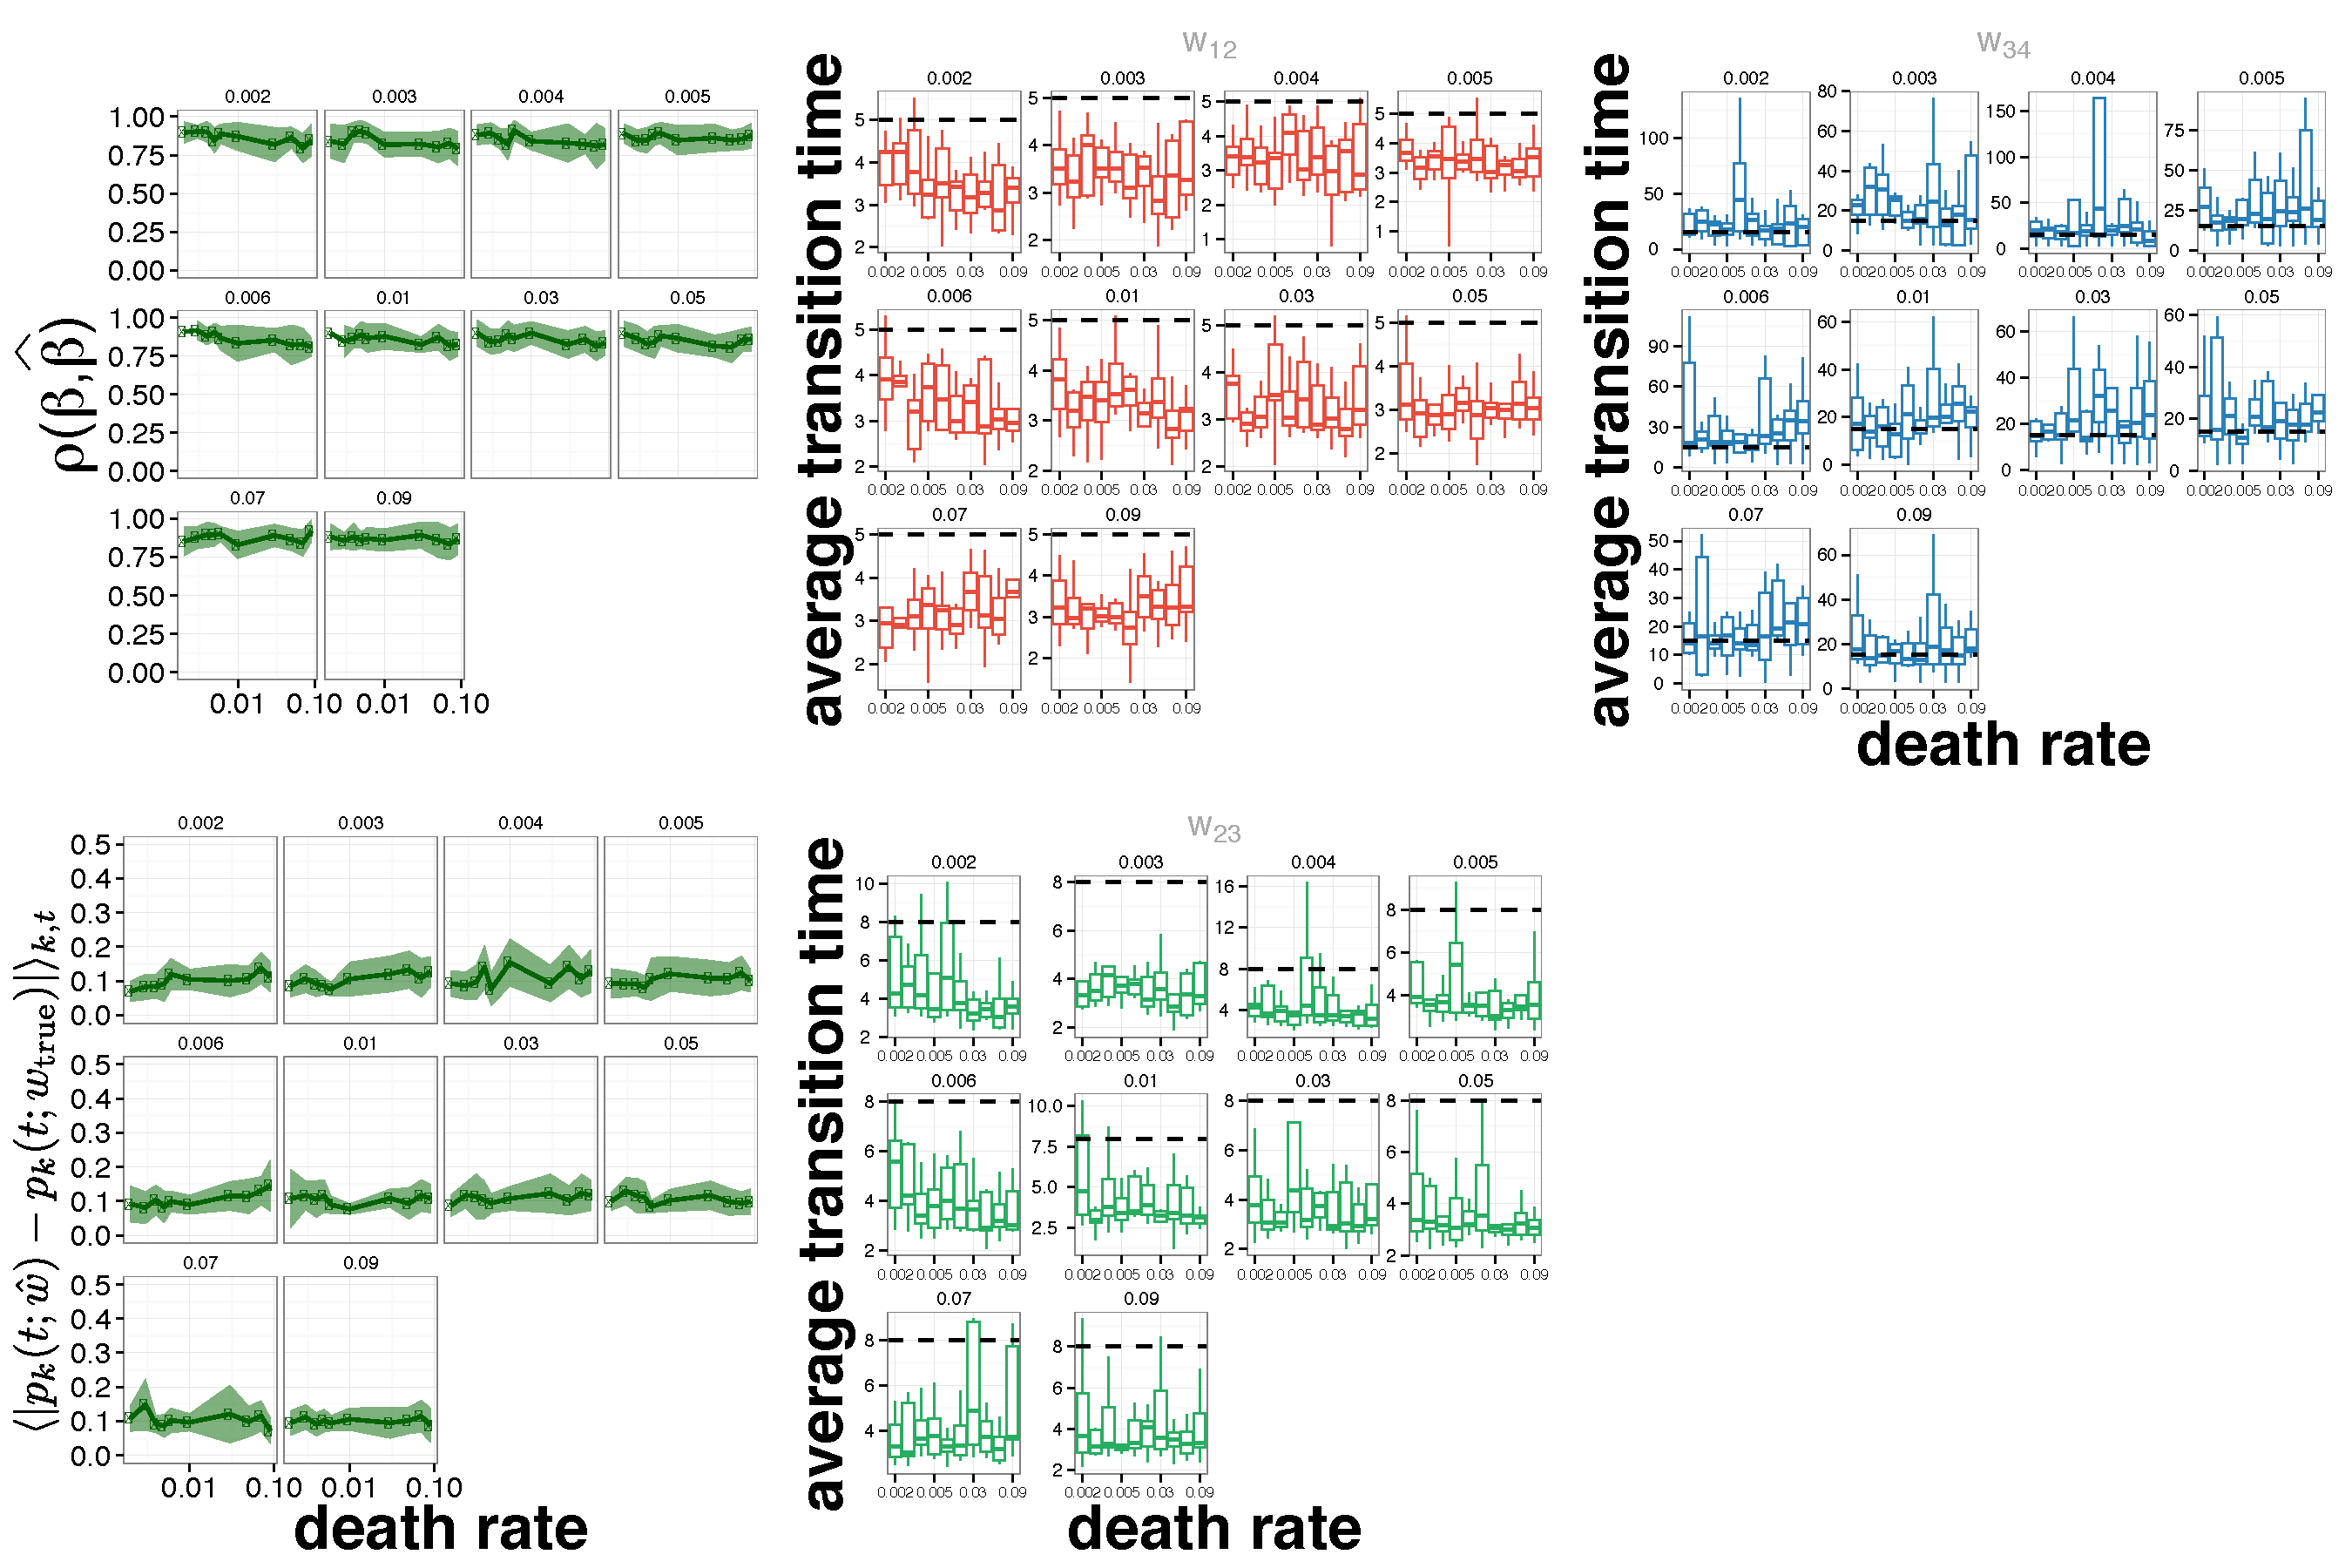
\includegraphics[width=0.9\textwidth]{pics/devide-2.pdf}
    \caption{Simulation study. Extend figure \ref{fig:dupl-realistic} to include a wider range of doubling rate. The top
left panel shows the correlations between true and estimated $\beta_{kj}$ as a function of death rates. The bottom left
panel shows the mean differences between estimated and true probabilities averaged over $10$ trajectories as a solid
line and the shaded area represents the standard deviation.Different panels show a range of doubling rates. The
remaining panels show boxplots for the estimated average transition times the horizontal dashed line shows the true
values used in estimation. }
    \label{fig:dupl-all}
\end{figure}


\begin{figure}
  \centering
  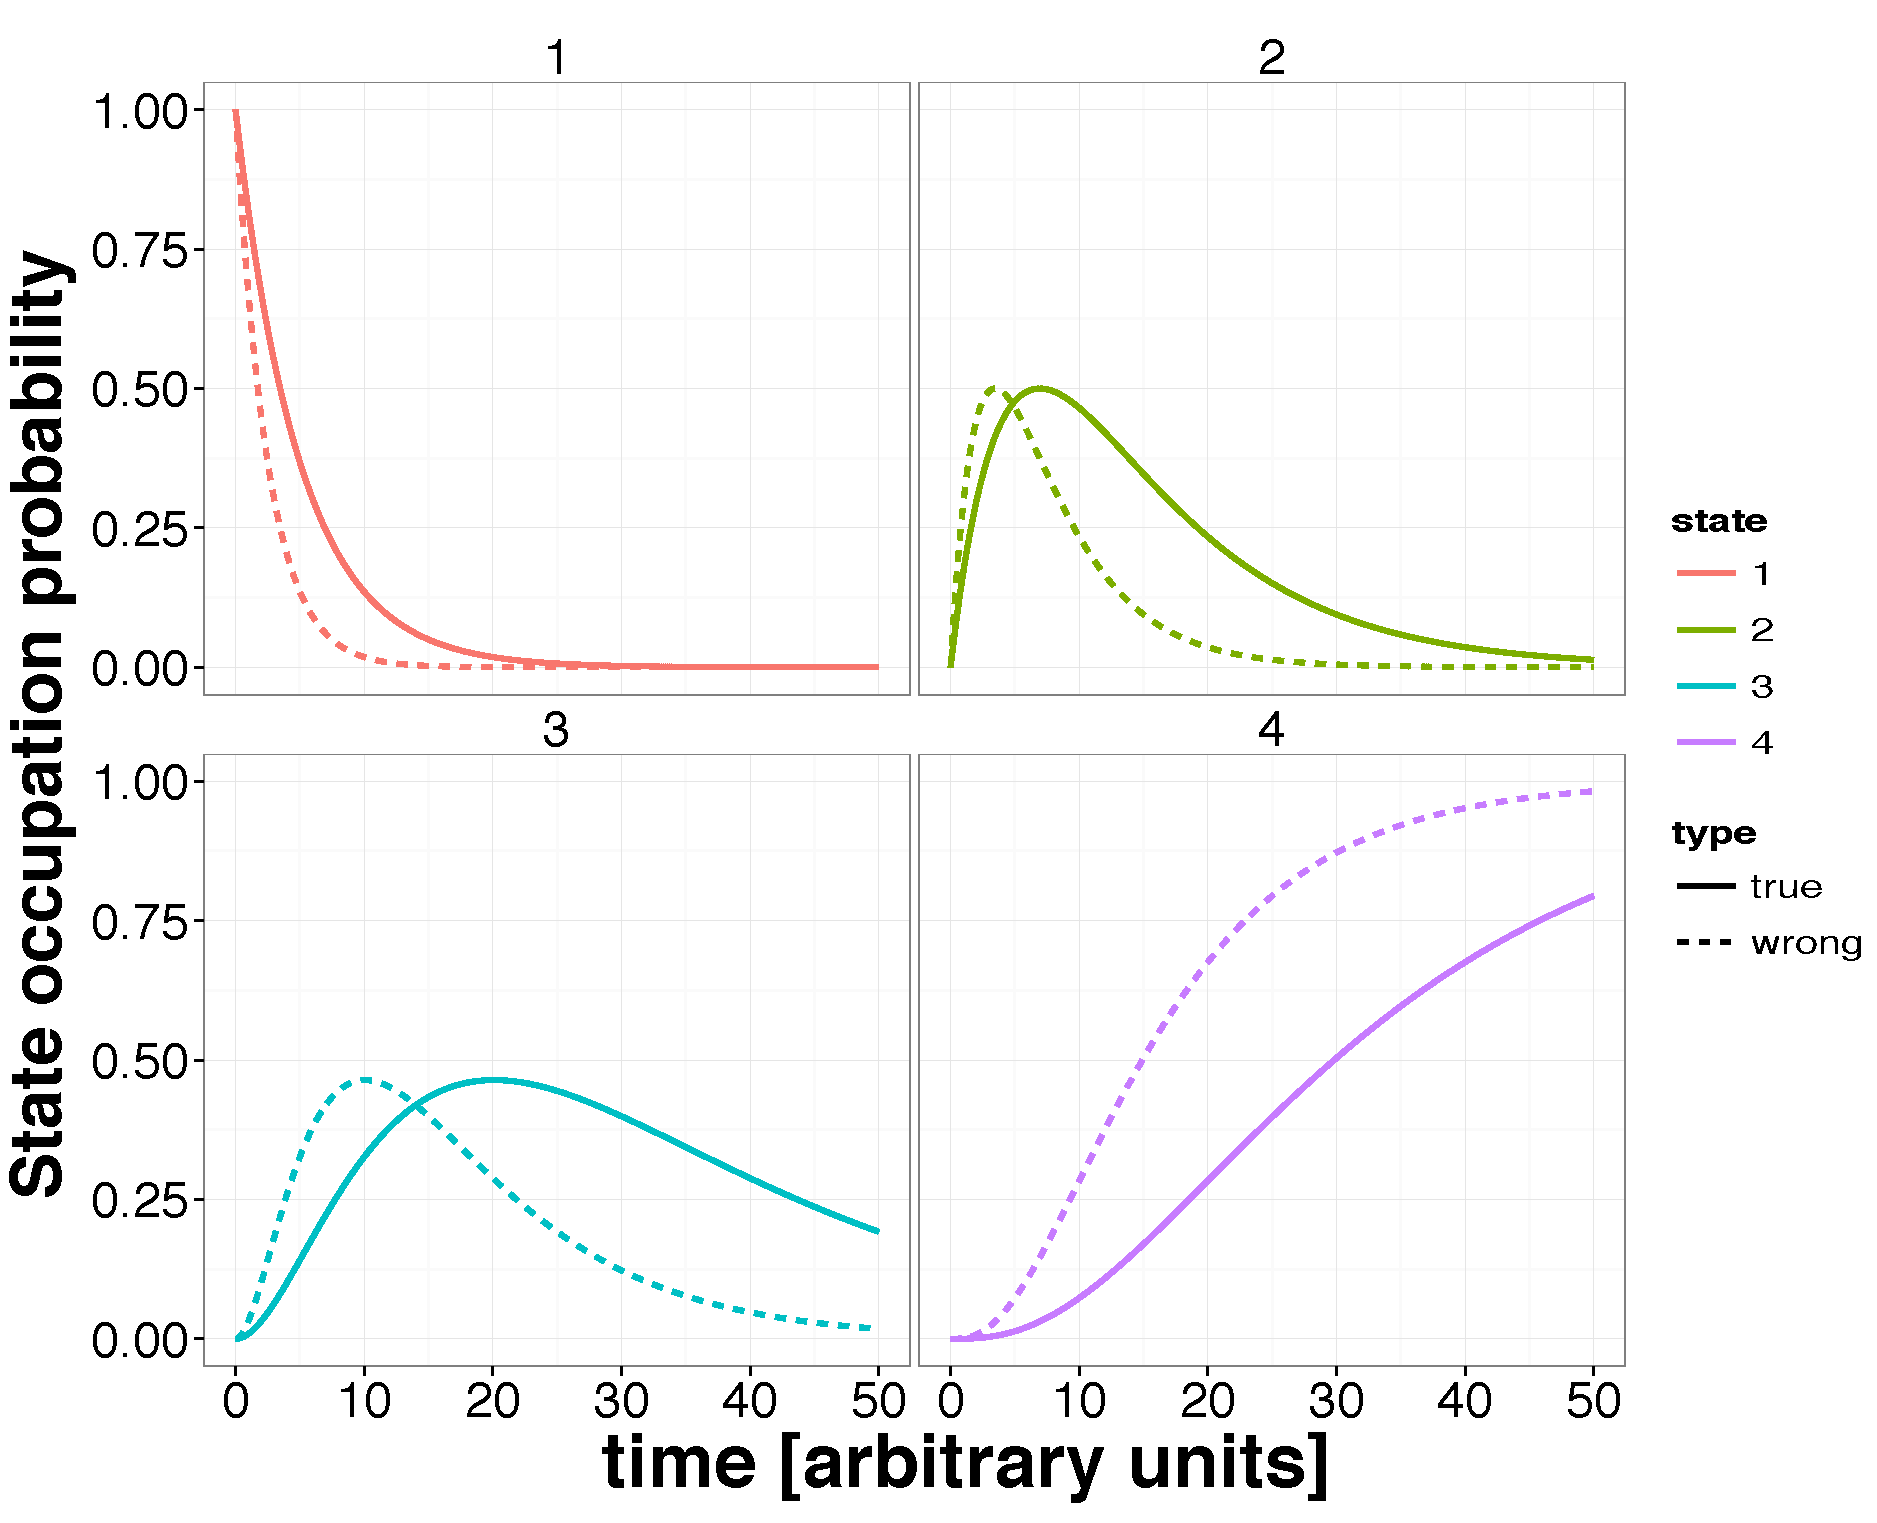
\includegraphics[width=0.8\textwidth]{pics/wrong_w.pdf}
  \caption{Simulation study. To highlight the effect of badly estimated}
  \label{fig:wrong_w}
\end{figure}


%%% Local Variables:
%%% TeX-master: "warwickthesis"
%%% End:
